\chapter{Creating a new test}
HULTI-GEN provides a step-by-step, test creation setup assistant. This assistant guides you through selecting a test method appropriate for your experiment, setting the parameters for your chosen method, customising the interface\footnote{Currently only available for grading tests}, adding stimuli, and assigning the stimuli into sessions and groups.
\newline\newline
To create a new test, from the main menu you first see when you first open HULTI-GEN, click the 'Create' button.

\begin{figure}[ht]
	\centering
	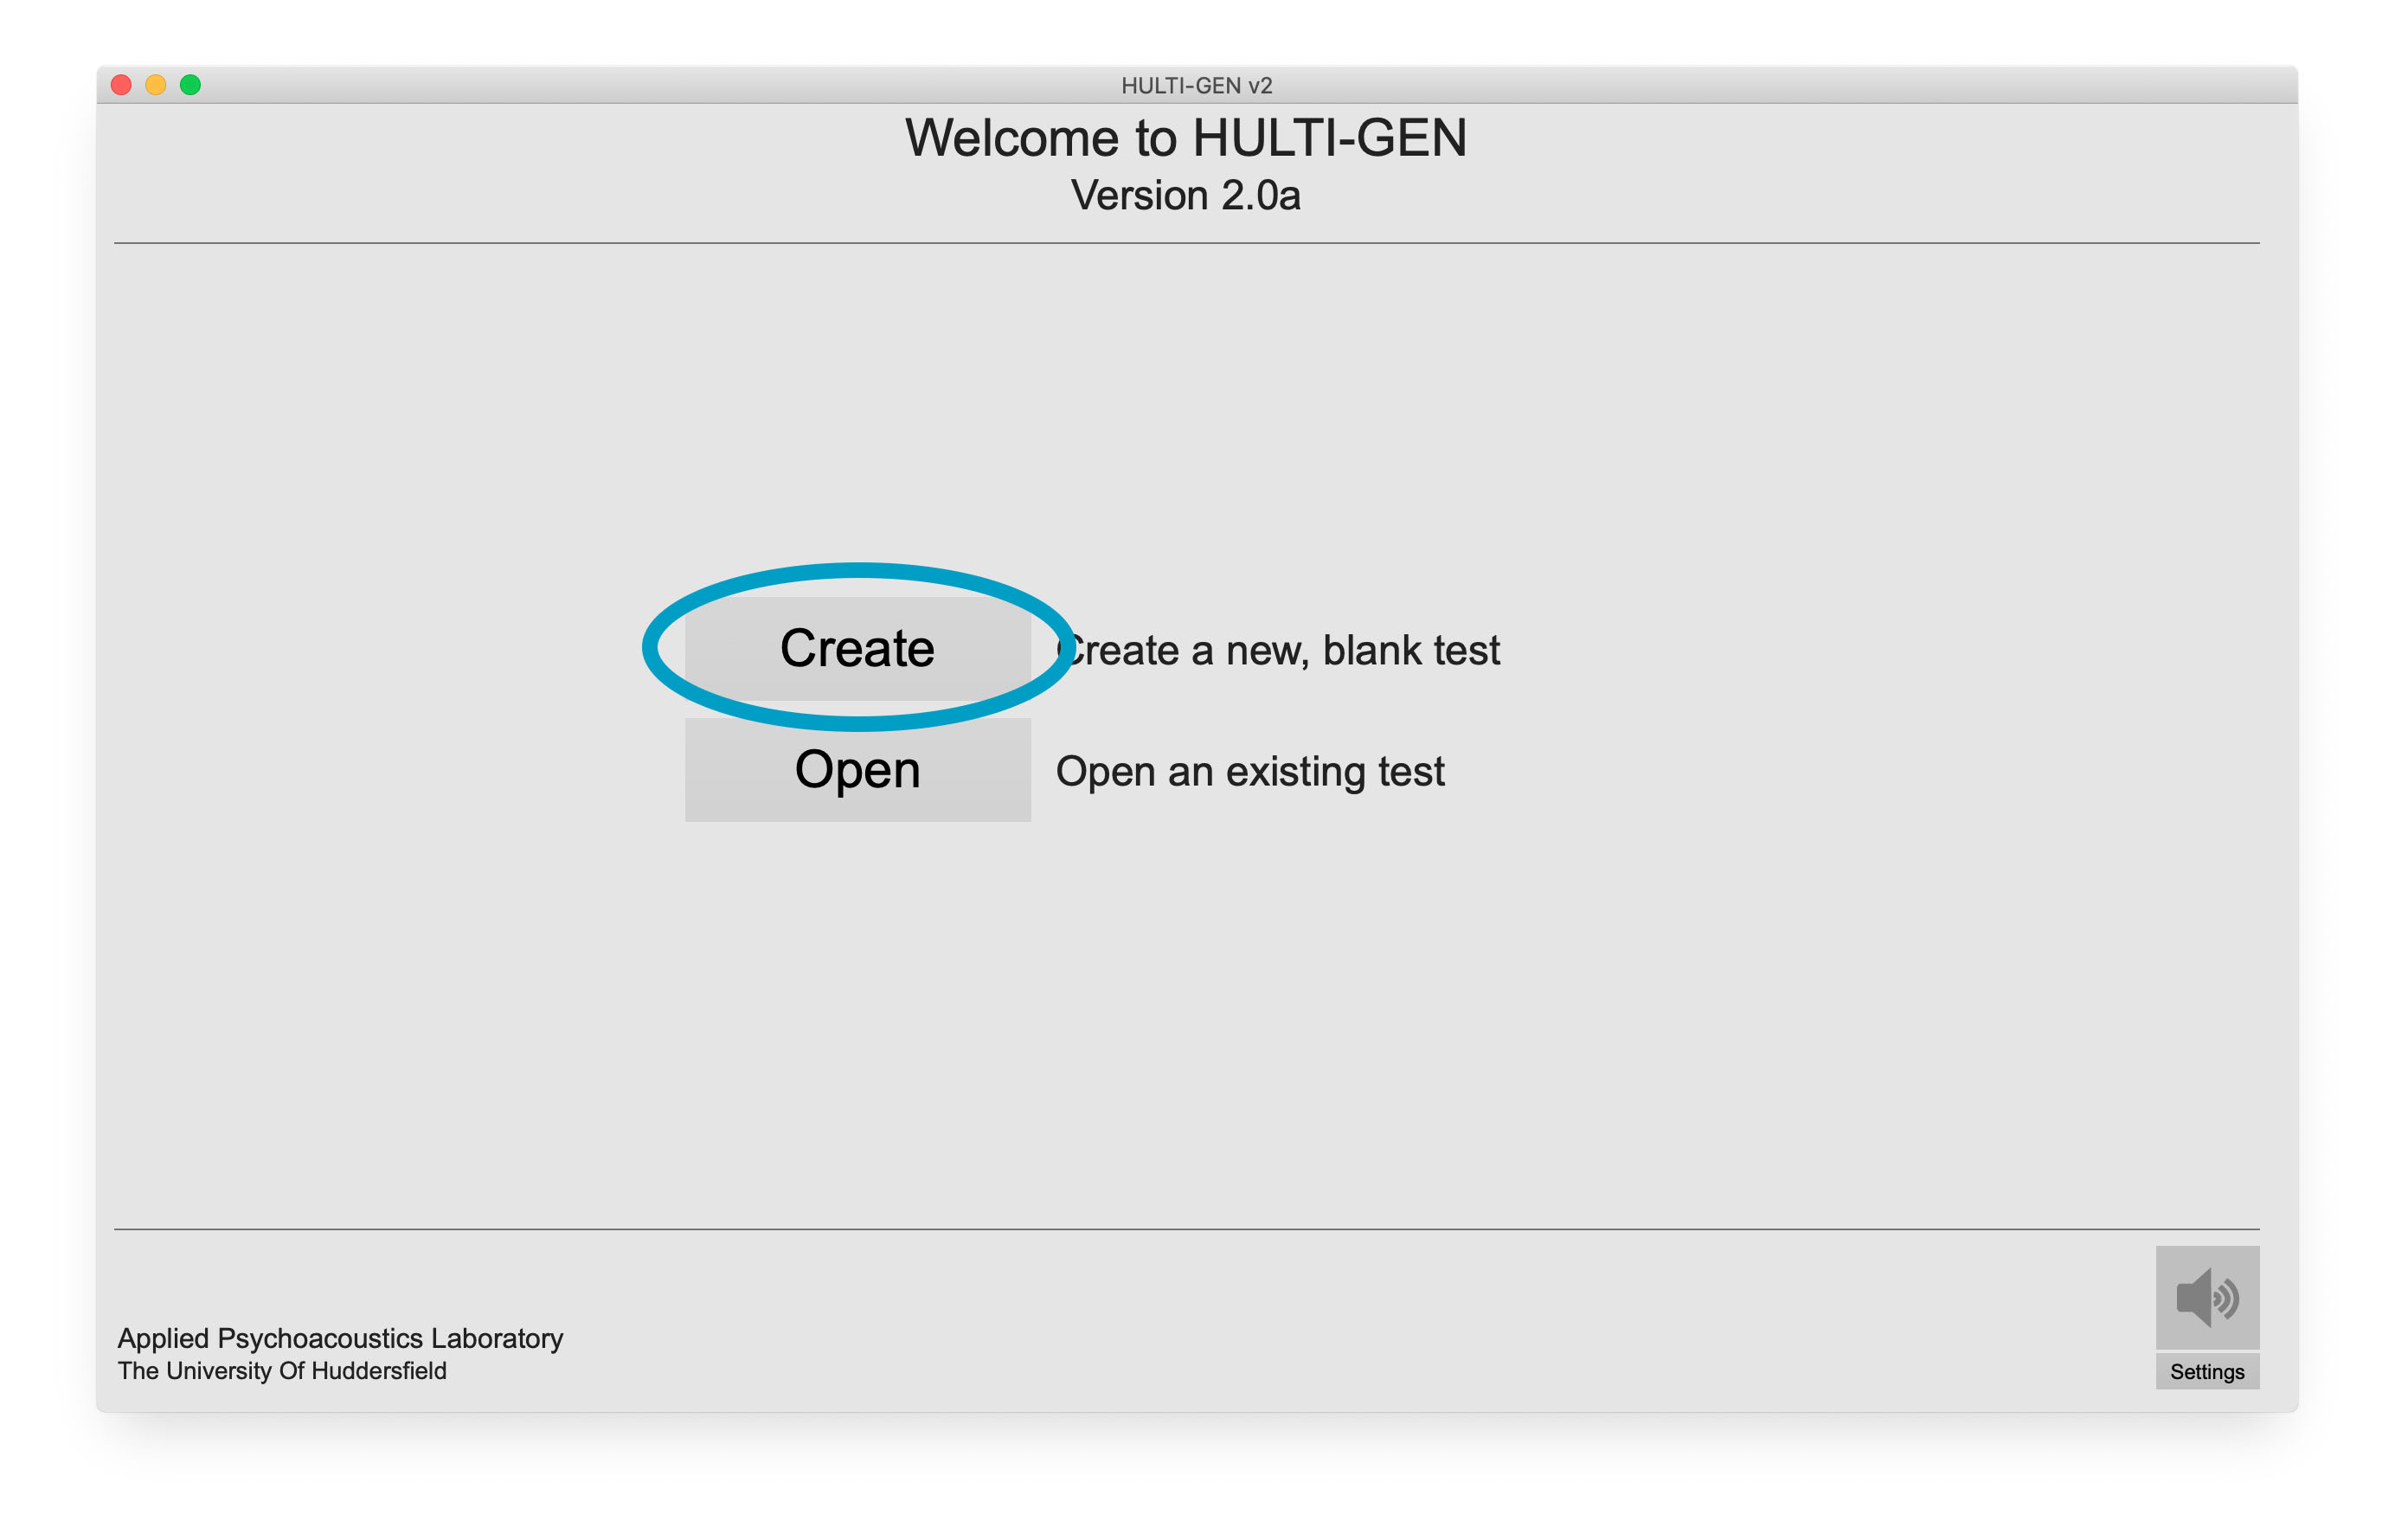
\includegraphics[width=1.0\textwidth]{./images/createTest_step01_mainScreen.jpg}
	\caption{Click on the 'Create' button to begin the test setup assistant.}
\end{figure}

\section{Step 1 - Test method setup}
Each test method available in HULTI-GEN is grouped by \emph{Procedure} and \emph{Task}. Procedure groups each task by its testing process. There are currently three available procedures:
\begin{itemize}
	\item Grading
	\item Non-adaptive psychophysical
	\item Adaptive psychophysical
\end{itemize}
 Task is specific task the subjects will carry out during the experiment, e.g. MUSHRA.

\section{Step 2 - Customising the test interface}

\section{Step 3 - Loading and assigning stimuli}